\documentclass{article}

\usepackage[spanish]{babel}
\usepackage[numbers,sort&compress]{natbib}
\usepackage[T1]{fontenc}
\usepackage[ansinew]{inputenc}
\usepackage{graphicx}
\usepackage{url}
\usepackage{caption}
\usepackage{subcaption}
\usepackage{float}

\title { Diagramas de Voronoi}
\author{Oscar Qui\~nonez}

\begin{document}

\maketitle
 
\section{Objetivo}\label{met}

En el presente trabajo se realiza la representaci\'on de una celda en la cual se siembran semillas, a trav\'es de la simulaci\'on usando Python, se intenta ver el comportamiento de las grietas formadas en esta celda, as\'i tambi\'en, determinar la mayor distancia euclidiana en una grieta.

\section{Metodolog\'ia}\label{met}

Dadas las instrucciones \cite{satuelisa} en la tarea 4, y el uso del c\'odigo \cite{baz}como referencia, se nos indica el uso de los diagamas de Voronoi, mediante la cual se gener\'o un c\'odigo que simulara la celda con variaciones en la cantidad de semillas, las cuales fueron, 40, 60, y 80 semillas.  

\section{Resultados y Discusi\'on}\label{res}

Al usar el c\'odigo generado, y variando la cantidad de semillas que se simularon en el diagrama de Voronoi con las cantidades dadas anteriormente, nos da como resultado una serie de im\'agenes de que representan la celda y cada color representa un espacio que ocupa la semilla, entre ellas, se forma una grieta que se puede apreciar en color negro y a medida que va creciendo, se va acercando al borde de la celda (figuras 1, 2 y 3).
En la figura 4 se pude apreciar que las celdas en las que se llega al borde son: 17, 21, 24, 25 y 26. Y que las distancias m\'aximas de recorrido fueron aproximadamente 80 celdas.
A continuaci\'on se muestran las figuras 5 y 6 en las que las distancias m\'aximas fueron mayor a 100 y aproximado a 70 respectivamente.

\begin{figure}[H]
       \centering
       \begin{subfigure}[b]{0.45\linewidth}
           
\includegraphics[width=\linewidth]{40semillas_15.png}
           \caption{Figura 1: celda con 40 semillas.}
           \label{fig:westminster_lateral}
        \end{subfigure}
        \begin{subfigure}[b]{0.45\linewidth}
            
\includegraphics[width=\linewidth]{60semillas_16.png}
            \caption{Figura 2: celda con 60 semillas.}
            \label{fig:westminster_aerea}
        \end{subfigure}
        \begin{subfigure}[b]{0.45\linewidth}
           
\includegraphics[width=\linewidth]{80semillas_15.png}
           \caption{Figura 3: celda con 80 semillas.}
           \label{fig:westminster_aerea}
        \end{subfigure}
        \begin{subfigure}[b]{0.45\linewidth}
           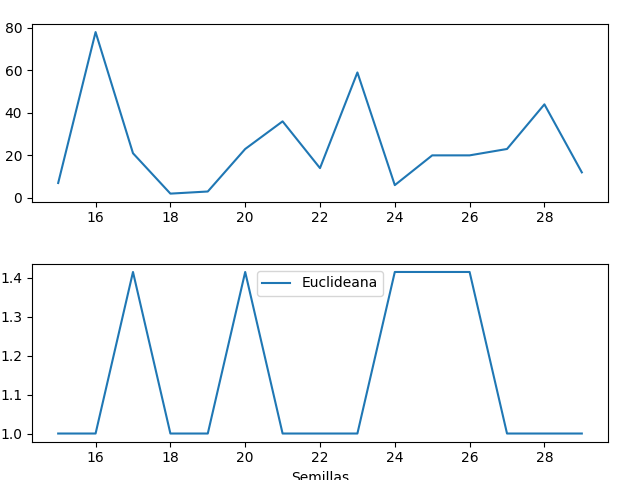
\includegraphics[width=\linewidth]{figura40semillas.png}
           \caption{Figura 4: celda con 40 semillas.}
           \label{fig:westminster_aerea}
        \end{subfigure}
      \begin{subfigure}[b]{0.45\linewidth}
           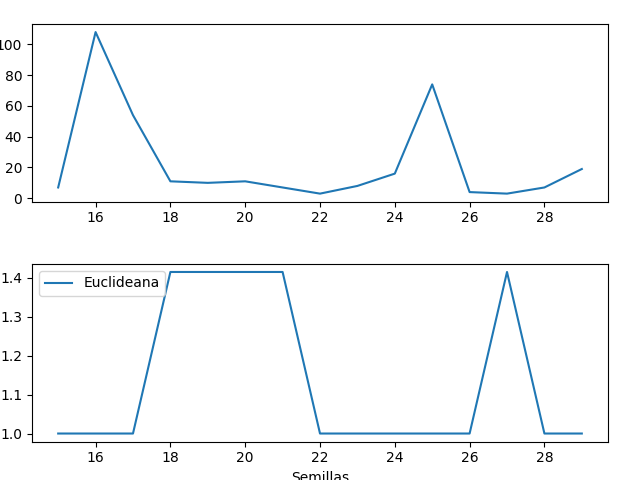
\includegraphics[width=\linewidth]{figura60semillas.png}
           \caption{Figura 5: celda con 60 semillas.}
           \label{fig:westminster_aerea}
        \end{subfigure}
\begin{subfigure}[b]{0.45\linewidth}
           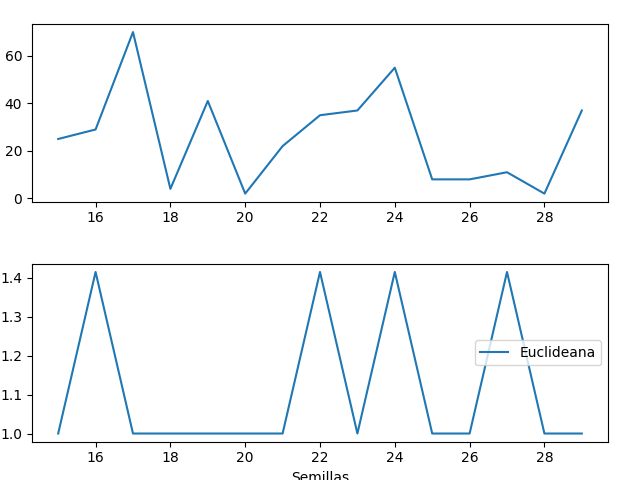
\includegraphics[width=\linewidth]{figura80semillas.png}
           \caption{Figura 6: celda con 80 semillas.}
           \label{fig:westminster_aerea}
        \end{subfigure}
\end{figure}

\newpage

\section{Conclusi\'on}

En las figura 7  y 8 vemos de mejor manera la diferencia entre el comienzo de una grieta y el final de la misma, lo que nos muestra claramente la distancia que recorri\'o.
Mediante el uso de los diagramas de Voronoi, se pudo determinar visualmente el comportamiento de las semillas dentro de una celda en la que va desarroll\'andose una grieta, por esta raz\'on es muy \'util este tipo de diagramas para la representaci\'on de un plano eucl\'ideo.
Todas las im\'agenes se pueden ver \cite{yo} en las carpetas destinadas para las distintas cantidades de semillas.

\begin{figure}[H]
       \centering
       \begin{subfigure}[b]{0.45\linewidth}
           
\includegraphics[width=\linewidth]{40semillas_15.png}
           \caption{Figura 7: inicio de la grieta.}
           \label{fig:westminster_lateral}
        \end{subfigure}
        \begin{subfigure}[b]{0.45\linewidth}
           
\includegraphics[width=\linewidth]{40semillas_23.png}
           \caption{Figura 8: fin de la grieta.}
           \label{fig:westminster_aerea}
        \end{subfigure}
\end{figure}

\bibliography{tareacuatro}
\bibliographystyle{unsrtnat}


\end{document}